\section{Experiment Results\label{sec:results}}

%when the available clues for alignment are sparse, we have performed comparative evaluation of our model against several baselines.


\subsection{Overall Performance\label{overall}}

\cparagraph{Results on $\bf DBP15K_{FR-EN}$} Table~\ref{cross} reports the results of all the compared approaches on $DBP15K_{FR-EN}$
dataset. We apply each approach
 to two alignment directions: French to English and vice versa. This dataset requires us to handle
cross-lingual data through rough machine translation which is likely to introduce lots of noise. We report the performance of JAPE on the
two implementations presented at
 ~\cite{sun2017cross} when using structure embedding (SE), and structure and attribute joint embedding (SE+AE).
Because JAPE uses the largest amount of annotated data (see Table~\ref {seed}), we expect it to give the best performance. As such, it
comes as no surprise that JAPE gives the highest Hits@10 scores. Our approach, \HRGCN (SE+AE), gives the second-best performance albeit it
uses significantly less annotated data. If we consider  Hit@1, a more important metric in practice, \HRGCN (SE+AE) outperforms all
alternative schemes with the highest Hit@1 score, which translates to an improvement of 38\% over JAPE (SE+AE). This is due to the
capability of \HRGCN (SE+AE) in preventing noisy nodes from driving the \KG representations. This experiment shows that our approach can
deliver comparable or even better performance compared to the best-performing prior method, but it achieves this using much less annotated
information and thus has a lower cost.



\cparagraph{Results on WBD} Table~\ref{f1} reports the performance of all models on WBD dataset. While the vanilla \GCN performs worse than
ITransE$'$, by adding highway gates to control the noise, \HGCN is able to outperform all existing approaches. By introducing highway gates
and pre-defined node features to the \RGCN, our \HRGCN (SE+AE) model delivers the best Hits@k score in both alignment directions, improving
upon ITransE$'$ by 38.9\% and 41.6\% for Hits@1 and Hits@10, respectively in the direction of Baidu$\rightarrow$Wiki. This shows that our
model has a distinct advantage in entity alignment over existing approaches.

\begin{table}
	\centering
	% \small
	\scriptsize
	\begin{tabular}{lrrrr}
		\toprule
		\multirow{2}{*}{$\bf DBP15K_{FR-EN}$} & \multicolumn{2}{c|}{$\bf FR \rightarrow EN$} & \multicolumn{2}{c}{$\bf EN \rightarrow FR$} \\
		& \bf Hits@1 & \bf Hits@10 & \bf Hits@1 & \bf Hits@10 \\
		\midrule
		\rowcolor{Gray}JE & 15.3 & 38.8 & 14.6 & 37.2 \\
		ITransE$'$ & 14.9 & 31.5 & 13.6 & 29.8 \\
		\rowcolor{Gray}MTransE & 24.4 & 55.5 & 21.2 & 50.6 \\
		JAPE (SE) & 29.6 & 64.5 & 26.5 & 60.3 \\
		\rowcolor{Gray}JAPE (SE+AE) & 32.3 & \bf 66.6 & 32.9 & \bf 65.9 \\
		\GCN & 15.3 & 32.1 & 13.6 & 31.9 \\
		\rowcolor{Gray}\HGCN & 19.6 & 36.9 & 18.4 & 35.5 \\
		\RGCN & 30.5 & 33.7 & 29.4 & 31.8 \\
		\rowcolor{Gray}\bf \HRGCN (w/o $X$) & 27.1 & 31.9 & 27.1 & 32.4 \\
		\bf \HRGCN (SE) & 33.4& 35.7& 31.2& 34.6 \\
		\rowcolor{Gray} 	\bf \HRGCN (SE+AE) & \bf 44.8 & 56.6 &\bf 41.0 & 52.9 \\
		\bottomrule
	\end{tabular}
	\caption{Performance on $DBP15K_{FR-EN}$ dataset.}
	\label{cross}
\end{table}

\begin{table}
	\centering
	% \small
	\scriptsize
	\begin{tabular}{lrrrr}
		\toprule
		\multirow{2}{*}{\bf WBD} &  \multicolumn{2}{c|}{$\bf Baidu \rightarrow Wiki$} & \multicolumn{2}{c}{$\bf Wiki \rightarrow Baidu$} \\
		& \bf Hits@1 & \bf Hits@10 & \bf Hits@1 & \bf Hits@10 \\
		\midrule
		\rowcolor{Gray} JE & 14.8 & 21.6 & 13.2 & 20.3 \\
		ITransE$'$ & 19.4 & 25.5 & 17.6 & 24.8 \\
		\rowcolor{Gray} \GCN & 17.1 & 27.3 & 15.7 & 25.9 \\
		\HGCN & 19.5 & 29.6 & 19.4 & 29.5  \\
		\rowcolor{Gray} \RGCN & 37.3 & 51.5 & 34.8 & 51.6 \\
		\bf \HRGCN (w/o $X$) & 15.0 & 21.7 & 14.5 & 21.5 \\
		\rowcolor{Gray} \bf \HRGCN (SE) & 50.7 & 64.3 & 49.2 & 62.6 \\
		\bf \HRGCN (SE+AE) & \bf 58.3 & \bf 67.1 & \bf 57.8{\tiny } & \bf 65.7 \\
		\bottomrule
	\end{tabular}
	\caption{Performance on WBD dataset.}
	\label{f1}
\end{table}

\subsection{Comparing Different Approaches\label{sec:analysis}}


%An extra advantage of GCN is that we can stack multiple convolution layers to capture more global and larger contextual and neighboring characteristics

%We now provide a detailed analysis to compare different approaches.

\cparagraph{\GCN vs. prior methods} Both  \GCN and JE only rely on aligned entities but not aligned relations or triples.  On WBD dataset,
the vanilla \GCN model outperforms JE for Hits@1 and Hits@10, and performs better than ITransE$'$ on Hits@10 for both alignment directions.
On the $DBP15K_{FR-EN}$ dataset, the \GCN outperforms ITransE$'$ in both directions. The performance improvement is largely due to the more
powerful graph modeling capability of \GCNs. Specifically, a \GCN emoploys convolutional layers to characterize an entity through careful
investigations about its neighbors, including both neighboring entities and attribute values; and as a result, it can provide more accurate
modeling and representation for the target entity.

\cparagraph{\GCN vs. \RGCN} As shown in Tables~\ref{f1} and ~\ref{cross}, an \RGCN further further improve the \GCN on both datasets. The
results suggest that introducing highly multi-relational information to the \GCN framework can improve the quality of the \KG
representations.


\cparagraph{(SE+AE) vs. (SE)} When comparing \HRGCN (SE+AE) with  \HRGCN (SE), we can see that adding attribute embedding greatly improves
the performance. This strategy leads to an increase of 11.4\%  in Hits@1 and 20.9\% in Hits@10 in the direction of FR$\rightarrow$EN in
Table~\ref{cross}. The results reinforce our claim that attribute information is crucially important for entity alignment and should not be
ignored. When comparing our full model \HRGCN with \HRGCN (w/o $X$) in Tables~\ref{cross} and ~\ref{f1}, we observe that removing
semantic/attribute information, $X$, from node representations leads to drops of over 20\% on the $DBP15K_{FR-EN}$ dataset and over 40\% on
the WBD dataset. The results indicate that it is crucial to utilize as much semantic and attribute information as possible to better
characterize entities in heterogeneous \KGs.
%initializing entity representations using pre-trained word embeddings and normalized attribute vectors is very helpful in aligning entities from different KGs.

\subsection{Sparse Alignment Clues}
To further investigate our model in more tough scenarios,
we divide the WBD dataset into four subsets according to the difference between the number of neighbors of each entity pair; we then compare the performance (in Hits@1) of ITransE$'$,  \GCN and \HRGCN (SE+AE). %on the four subsets.
The results are given in Figure~\ref{subset}.

When the number of neighbors differs by no more than 2, the Hits@1 score of all three models are over 20\%. When the difference between the
entity pairs' neighborhood becomes more prominent, \HRGCN (SE+AE) tends to deliver more stable performance, with slower drop in Hits@1
compared to \GCN and ITransE$'$. When the difference of neighborhood is larger than 9, \HRGCN (SE+AE) still maintains over a in Hits@1
score of 37, with a performance drop of 35\%. By contrast, both ITransE$'$ and \GCN only give a Hits@1 score of less than 10, which
translates to over a performance drop of over 50\% when the number of neighbors differs by no more than 2. The more stable performance of
our \HRGCN model is largely attributed to the introduction of highway gates, which can help the model better embed the relational structure
information and focus on the most discriminative aspects from the target entity's neighbors.


\begin{figure}
	\centering
	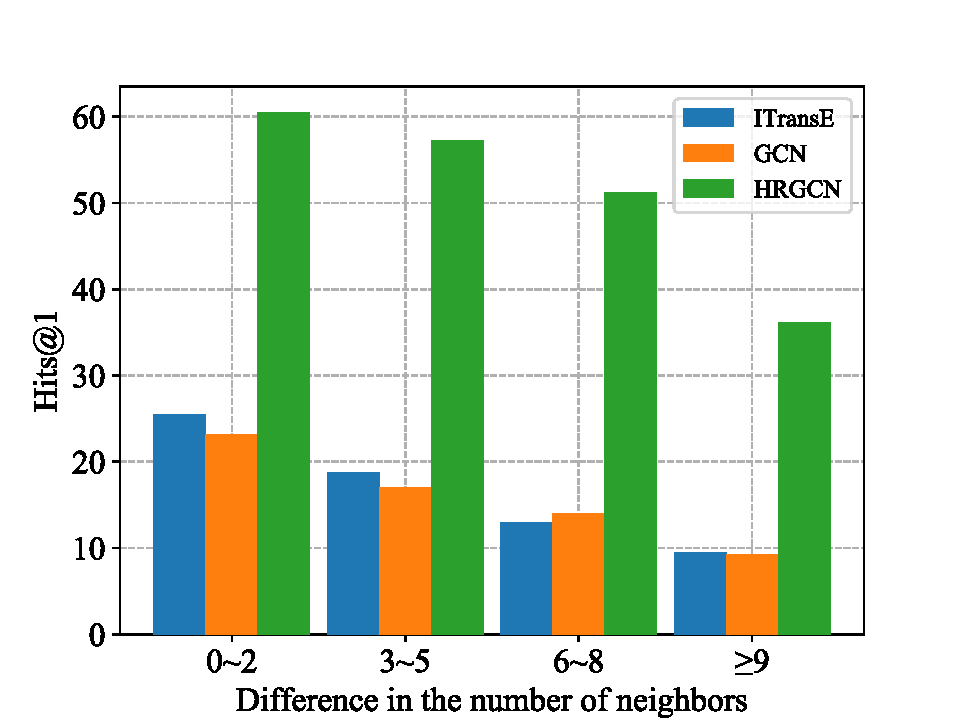
\includegraphics[width=1\linewidth]{figures/graph4.pdf}
	\caption{Hits@1 scores for ITransE$'$, \GCN and \HRGCN (SE+AE) on the four WBD subsets. The number range, $x\sim y$, on the
x-axis denotes the the subset in which the number of neighbors differs from $x$ to $y$ for each entity pair.}
	\label{subset}
\end{figure}

Moreover, we randomly select several examples from the WBD dataset (see Table~\ref{example}), as well as their neighbor information, i.e.,
the number of neighbors, values, potentially overlapped neighbors or values for each pair. We can find that although some entities have
dozens of neighbors in their own \KGs,  there is only a small number of potentially overlapped neighbors. This confirms our motivation that
the available clues for entity alignment are sparse (see Section~\ref{sec:motivation}). Due to the working mechanism of the models,
  ITransE$'$ fails to locate discriminative neighbors but \HRGCN (SE+AE) can still identify useful structure information from such limited clues.
We also observe that attribute values play an important role in entity alignment. For instance, in the entity pair of \textit{Hubei
Province}, nearly half of the neighbors for each entity are values. Among 3 out of the 5 similar neighbors are actually values, which
provide crucial supporting evidence for successful alignment. Unfortunately, ITransE$'$ cannot utilize those information, thus is unable to
correctly algin this entity.

\begin{table}
	\centering
	\scriptsize
	\begin{tabular}{lcrcr}
		\toprule
		\multirow{2}{*}{\bf Aligned Entities} & \bf \#Neighbors & \bf \#Similar & \bf \#Values & \bf \#Similar \\
		&\bf  Wiki \& Baidu &\bf  Neighbors &\bf  Wiki \& Baidu &\bf  Values \\
		\midrule
		Deng Jiaxian & 10 \& 33 & 5 & \ 3 \& 11 & 2\\
		Hubei Province & 21 \& 50 & 5 & 10 \& 19 & 3\\
		European Union & 66 \& 35 & 6 & 18 \& 8\ \ \ & 2\\
		%Huazhong University of & \multirow{2}{*}{11 \& 32} & \multirow{2}{*}{4} & \multirow{2}{*}{8 \& 6} & \multirow{2}{*}{1}\\
		%Science and Technology & & & & \\
		%Huazhong University of Science and Technology & 11 \& 32 & 4 & 8 \& 6 & 1 \\
		Confucius & 10 \& 20 & 4 & 7 \& 3 & 2\\
		\bottomrule
	\end{tabular}
	\caption{The statistics of example entity pairs, which our \HRGCN(SE+AE) model correctly aligns but ITransE$'$ fails.}
	\label{example}
\end{table}


\subsection{Impact of Highway Gates} Intuitively, adding more \HRGCN layers can help the target entities obtain information from neighbors that are multiple hops
further away. However, doing so might also introduce noisy information from the exponentially increasing neighbors, leading to significant
decline in performance. This observation is illustrated in Figure~\ref{highway}, where we compare our model with different numbers layers
with (\emph{+highway}) and without (\emph{-highway}) highway gates. We can observe that the performance of two-layered \RGCNs with highway
gates improves upon the one-layered \RGCN. After that point, adding more layers to the \RGCN will lead to performance depredation, but the
performance of the highway \RGCNs decreases slower than the non-highway-gate counterparts. This confirms our claim that the highway gates
can effectively control neighbor information pass through \RGCN layers to control the noise. 

In addition, from Table~\ref{f1}, we can see that the \GCN or \RGCN-based models with highway gates consistently achieve better performance than no-highway ones, indicating that highway gates can effectively improve the performance of both multi-layered \GCN and \RGCN models.
\begin{figure}
	\centering
	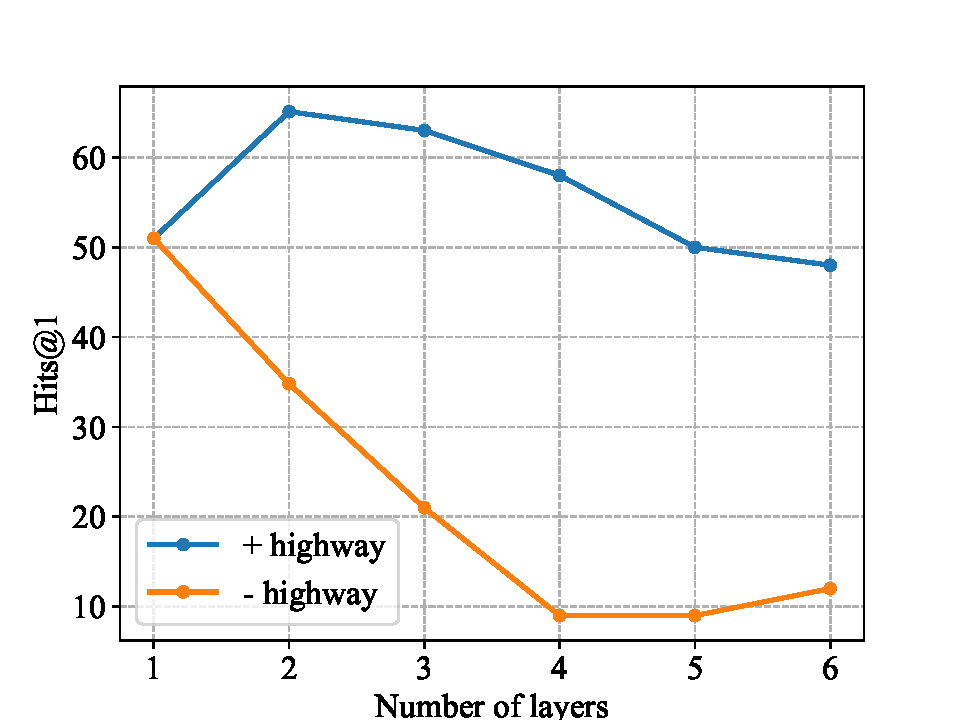
\includegraphics[width=0.9\linewidth]{figures/graph3.pdf}
	\caption{The effect of adding more \RGCN layers in terms of Hits@1 over the test set of WBD with and without the highway gates.}
	\label{highway}
\end{figure}
